\documentclass[11pt,a4paper]{jsarticle} %,uplatex
\usepackage{amsmath,amssymb}
\usepackage{amsthm}
\usepackage{ascmac}
\usepackage{bm}
\usepackage[dvipdfmx]{graphicx}	% required for `\includegraphics' (yatex added)
\usepackage{setspace}           % required for `\doublespace'
\usepackage{tikz}
\usepackage{tikz-cd}
\usetikzlibrary{angles, positioning, shapes, arrows.meta, decorations.pathmorphing}
%\usetikzlibrary{intersections, calc, arrows, positioning, arrows.meta}
\usepackage{tcolorbox}  % 定理環境の装飾
\tcbuselibrary{skins, breakable, theorems}
\usepackage{xcolor}
\usepackage{natbib}
\usepackage{pxrubrica}
\usepackage[margin=30truemm, left=40truemm, right=40truemm]{geometry}
\usepackage{thmbox}     % required for theorem environment with side bar
%
\setlength{\parskip}{3mm} %段落間にスペースを入れる


% \pagestyle{myheadings}
% \markright{\footnotesize \sf 2022秋期「哲学者のための数学」授業資料(大塚淳) \ \ 配布禁止}


\theoremstyle{definition}
\newtheorem[S]{exercise}{練習問題}[section]
\newtheorem[S]{example}{事例}[section]
\newtheorem[S]{fact}{事実}[section]
\newtheorem[S]{attn}{注意}[section]
\newtheorem[S]{develop}{発展}[section]
\renewcommand{\theattn}{}

\newtcbtheorem[auto counter, number within=section]{rei}{事例}{
    breakable,
    coltitle=black,
    fonttitle=\bfseries,
    enhanced, colback=white, frame hidden, borderline west = {0.5pt}{5pt}{black},
%    number freestyle={\noexpand\thesection.\noexpand\arabic{\tcbcounter}}
}{rei}

\newtcbtheorem[auto counter, number within=section]{prop}{命題}{
    breakable,
    coltitle=black,
    fonttitle=\bfseries,
    enhanced, colback=white, frame hidden, borderline west = {0.5pt}{5pt}{black},
%    number freestyle={\noexpand\thesection.\noexpand\arabic{\tcbcounter}}
}{prop}

\newtcbtheorem[number within=section]{renshu}{練習問題}{
    breakable,
    coltitle=black,
    fonttitle=\bfseries,
    enhanced, colback=white, frame hidden, borderline west = {0.5pt}{5pt}{black}
}{renshu}


\newtcbtheorem[number within=section]{hatten}{発展}{
    breakable,
    coltitle=black,
    fonttitle=\bfseries,
    enhanced, colback=white, frame hidden, borderline west = {0.5pt}{5pt}{black}
}{renshu}


\newtcbtheorem[number within=section]{dfn}{定義}{
    fonttitle=\bfseries,
    enhanced, colback=white
}{dfn}


% Bold face capital letters:
\newcommand{\bfzero}{\boldsymbol{0}}
\newcommand{\bfone}{\boldsymbol{1}}
\newcommand{\bfA}{\boldsymbol{A}}
\newcommand{\bfB}{\boldsymbol{B}}
\newcommand{\bfC}{\boldsymbol{C}}
\newcommand{\bfD}{\boldsymbol{D}}
\newcommand{\bfE}{\boldsymbol{E}}
\newcommand{\bfF}{\boldsymbol{F}}
\newcommand{\bfG}{\boldsymbol{G}}
\newcommand{\bfH}{\boldsymbol{H}}
\newcommand{\bfI}{\boldsymbol{I}}
\newcommand{\bfJ}{\boldsymbol{J}}
\newcommand{\bfK}{\boldsymbol{K}}
\newcommand{\bfL}{\boldsymbol{L}}
\newcommand{\bfM}{\boldsymbol{M}}
\newcommand{\bfN}{\boldsymbol{N}}
\newcommand{\bfO}{\boldsymbol{O}}
\newcommand{\bfP}{\boldsymbol{P}}
\newcommand{\bfQ}{\boldsymbol{Q}}
\newcommand{\bfR}{\boldsymbol{R}}
\newcommand{\bfS}{\boldsymbol{S}}
\newcommand{\bfT}{\boldsymbol{T}}
\newcommand{\bfU}{\boldsymbol{U}}
\newcommand{\bfV}{\boldsymbol{V}}
\newcommand{\bfW}{\boldsymbol{W}}
\newcommand{\bfX}{\boldsymbol{X}}
\newcommand{\bfY}{\boldsymbol{Y}}
\newcommand{\bfZ}{\boldsymbol{Z}}

\newcommand{\bfa}{\boldsymbol{a}}
\newcommand{\bfb}{\boldsymbol{b}}
\newcommand{\bfc}{\boldsymbol{c}}
\newcommand{\bfd}{\boldsymbol{d}}
\newcommand{\bfe}{\boldsymbol{e}}
\newcommand{\bff}{\boldsymbol{f}}
\newcommand{\bfk}{\boldsymbol{k}}
\newcommand{\bfm}{\boldsymbol{m}}
\newcommand{\bfn}{\boldsymbol{n}}
\newcommand{\bfo}{\boldsymbol{o}}
\newcommand{\bfp}{\boldsymbol{p}}
\newcommand{\bfq}{\boldsymbol{q}}
\newcommand{\bfr}{\boldsymbol{r}}
\newcommand{\bfs}{\boldsymbol{s}}
\newcommand{\bft}{\boldsymbol{t}}
\newcommand{\bfu}{\boldsymbol{u}}
\newcommand{\bfv}{\boldsymbol{v}}
\newcommand{\bfw}{\boldsymbol{w}}
\newcommand{\bfx}{\boldsymbol{x}}
\newcommand{\bfy}{\boldsymbol{y}}
\newcommand{\bfz}{\boldsymbol{z}}



% BB (???) capital letters:
\newcommand{\bbA}{\mathbb{A}}
\newcommand{\bbB}{\mathbb{B}}
\newcommand{\bbC}{\mathbb{C}}
\newcommand{\bbD}{\mathbb{D}}
\newcommand{\bbE}{\mathbb{E}}
\newcommand{\bbF}{\mathbb{F}}
\newcommand{\bbG}{\mathbb{G}}
\newcommand{\bbI}{\mathbb{I}}
\newcommand{\bbN}{\mathbb{N}}
\newcommand{\bbP}{\mathbb{P}}
\newcommand{\bbQ}{\mathbb{Q}}
\newcommand{\bbR}{\mathbb{R}}
\newcommand{\bbU}{\mathbb{U}}
\newcommand{\bbV}{\mathbb{V}}
\newcommand{\bbX}{\mathbb{X}}
\newcommand{\bbY}{\mathbb{Y}}
\newcommand{\bbZ}{\mathbb{Z}}
\newcommand{\bbone}{{\ifmmode\mathrm{1\!l}\else\mbox{\(\mathrm{1\!l}\)}\fi}}


% Caligraphic math capital letters:
\newcommand{\mcalA}{\mathcal{A}}
\newcommand{\mcalB}{\mathcal{B}}
\newcommand{\mcalC}{\mathcal{C}}
\newcommand{\mcalD}{\mathcal{D}}
\newcommand{\mcalE}{\mathcal{E}}
\newcommand{\mcalF}{\mathcal{F}}
\newcommand{\mcalG}{\mathcal{G}}
\newcommand{\mcalH}{\mathcal{H}}
\newcommand{\mcalI}{\mathcal{I}}
\newcommand{\mcalJ}{\mathcal{J}}
\newcommand{\mcalK}{\mathcal{K}}
\newcommand{\mcalL}{\mathcal{L}}
\newcommand{\mcalM}{\mathcal{M}}
\newcommand{\mcalN}{\mathcal{N}}
\newcommand{\mcalO}{\mathcal{O}}
\newcommand{\mcalP}{\mathcal{P}}
\newcommand{\mcalQ}{\mathcal{Q}}
\newcommand{\mcalS}{\mathcal{S}}
\newcommand{\mcalT}{\mathcal{T}}
\newcommand{\mcalU}{\mathcal{U}}
\newcommand{\mcalV}{\mathcal{V}}
\newcommand{\mcalX}{\mathcal{X}}
\newcommand{\mcalY}{\mathcal{Y}}
\newcommand{\mcalZ}{\mathcal{Z}}

% Graph nodes notations:
\newcommand{\PA}{\mathit{PA}}
\newcommand{\bfPA}{\mathbf{PA}}
\newcommand{\CH}{\mathit{CH}}
\newcommand{\bfCH}{\mathbf{CH}}
\newcommand{\DS}{\mathit{DS}}
\newcommand{\bfDS}{\mathbf{DS}}
\newcommand{\ND}{\mathit{ND}}
\newcommand{\bfND}{\mathbf{ND}}
\newcommand{\AN}{\mathit{an}}
\newcommand{\bfAN}{\mathbf{an}}
\newcommand{\pa}{\mathit{pa}}
\newcommand{\bfpa}{\mathbf{pa}}
\newcommand{\ch}{\mathit{ch}}
\newcommand{\bfch}{\mathbf{ch}}
\newcommand{\ds}{\mathit{ds}}
\newcommand{\bfds}{\mathbf{ds}}
\newcommand{\nd}{\mathit{nd}}
\newcommand{\bfnd}{\mathbf{nd}}
\newcommand{\an}{\mathit{an}}
\newcommand{\bfan}{\mathbf{an}}



\DeclareMathOperator*{\argmax}{arg\,max}
\DeclareMathOperator*{\argmin}{arg\,min}
\DeclareMathOperator*{\argsup}{arg\,sup}
\DeclareMathOperator*{\arginf}{arg\,inf}
\DeclareMathOperator{\erfc}{erfc}
\DeclareMathOperator{\diag}{diag}
\DeclareMathOperator{\cum}{cum}
\DeclareMathOperator{\sgn}{sgn}
\DeclareMathOperator{\tr}{tr}
\DeclareMathOperator{\spn}{span}
\DeclareMathOperator{\adj}{adj}
\DeclareMathOperator{\E}{\mathbb{E}}
\DeclareMathOperator{\var}{Var}
\DeclareMathOperator{\cov}{Cov}
\DeclareMathOperator{\corr}{corr}
\DeclareMathOperator{\sech}{sech}
\DeclareMathOperator{\sinc}{sinc}
\DeclareMathOperator*{\lms}{l.i.m.\,}
\newcommand{\varop}[1]{\var\left[{#1}\right]}
\newcommand{\covop}[2]{\cov\left({#1},{#2}\right)}
\newcommand{\T}{^\textrm{T}}
\newcommand\indep{\protect\mathpalette{\protect\independenT}{\perp}}
\def\independenT#1#2{\mathrel{\rlap{$#1#2$}\mkern2mu{#1#2}}}

\newcommand{\bfalpha}{\boldsymbol{\alpha}}
\newcommand{\bfbeta} {\boldsymbol{\beta}}
\newcommand{\bfgamma}{\boldsymbol{\gamma}}
\newcommand{\bfeta}  {\boldsymbol{\eta}}
\newcommand{\bftheta}{\boldsymbol{\theta}}
\newcommand{\bflambda}   {\boldsymbol{\lambda}}
\newcommand{\bfmu}   {\boldsymbol{\mu}}
\newcommand{\bfnu}   {\boldsymbol{\nu}}
\newcommand{\bfxi}   {\boldsymbol{\xi}}
\newcommand{\bfpsi}  {\boldsymbol{\psi}}
\newcommand{\bfphi}   {\boldsymbol{\phi}}
\newcommand{\bfrho}   {\boldsymbol{\rho}}
\newcommand{\bfvarepsilon}{\boldsymbol{\varepsilon}}
%\newcommand{\qed}{{qed}}
%\newcommand{\eqalignno}[1]{\begin{array}{ccccccc}#1\end{array}}

\newcommand{\bfGamma}{\boldsymbol{\Gamma}}
\newcommand{\bfTheta}{\boldsymbol{\Theta}}
\newcommand{\bfLambda}   {\boldsymbol{\Lambda}}
\newcommand{\bfPsi}  {\boldsymbol{\Psi}}
\newcommand{\bfPhi}   {\boldsymbol{\Phi}}
\newcommand{\bfSigma}  {\boldsymbol{\Sigma}}
\newcommand{\bfOmega}  {\boldsymbol{\Omega}}


% DISTRIBUTIOoNS: 
\newcommand{\normal}{\mathcal{N}}
\newcommand{\binomial}{\mathcal{B}}
\newcommand{\multinomial}{\mathcal{M}}
\newcommand{\exponential}{\mathcal{E}}
\newcommand{\geometric}{\mathcal{G}}
\newcommand{\poisson}{\mbox{Poisson}}
\newcommand{\uniform}{\mbox{Uniform}}

% Logic
\newcommand{\true}{\texttt{true}}
\newcommand{\false}{\texttt{false}}


%PSTricks (commande for latent nodes)
\newcommand{\lnode}[4]{ \cnode(#1){#2}{#3}\rput(#1){\footnotesize#4} }

% KEEPING TRACK OF WORK
\newcommand{\todo}[1]
{
{\color{red}{
[TODO: #1]}}
\addcontentsline{toc}{subsection}{TO DO: #1}
}

\newcommand{\fixme}[1]{{\color{red}{#1}}}

\newenvironment{answer}[1]
{\par \color{blue}{#1}}
{}


\newcommand{\note}[2]
{
{\color{red}{
[#1: #2]}}
}




\makeatletter
% define \citepos for posesive citation (e.g. Otsuka's (2015))
\DeclareRobustCommand\citepos
  {\begingroup
   \let\NAT@nmfmt\NAT@posfmt% ...except with a different name format
   \NAT@swafalse\let\NAT@ctype\z@\NAT@partrue
   \@ifstar{\NAT@fulltrue\NAT@citetp}{\NAT@fullfalse\NAT@citetp}}

\let\NAT@orig@nmfmt\NAT@nmfmt
\def\NAT@posfmt#1{\NAT@orig@nmfmt{#1's}}
\makeatother




% Code for drawing color circle used in topology (pathconnectedness)
\usepackage{xparse}
\ExplSyntaxOn

\keys_define:nn { colour_transition_circle } {
    inner   .fp_set:N   = \l__inner_radius,
    inner   .initial:n  = {2},
    outer   .fp_set:N   = \l__outer_radius,
    outer   .initial:n  = {3},
    angle   .fp_set:N   = \l__start_angle,
    angle   .initial:n  = {0}
}

\NewDocumentCommand \ColourTransitionCircle { O{} m } {
\group_begin:
    \keys_set:nn { colour_transition_circle } {#1}
    \clist_clear:N \l_tmpa_clist
    \clist_map_inline:nn {#2} {
        \clist_put_right:Nn \l_tmpa_clist {##1}
        %\clist_put_right:Nn \l_tmpa_clist {##1}
    }
    \exp_args:Nx \col_trans_circ:n \l_tmpa_clist
\group_end:
}

\cs_new_protected:Npn \col_trans_circ:n #1 {
    \int_step_inline:nnnn {1} {1} {\clist_count:n {#1} - 1} {
        \path[top~color=\clist_item:nn {#1} {##1}, bottom~color=\clist_item:nn {#1} {##1+1}, shading~angle={270-(180-360/\clist_count:n {#1})/2+(##1-1)*360/\clist_count:n {#1}+\fp_use:N \l__start_angle}] ({\fp_use:N \l__inner_radius*cos((##1-1)*360/\clist_count:n {#1}+\fp_use:N \l__start_angle)},{\fp_use:N \l__inner_radius*sin((##1-1)*360/\clist_count:n {#1}+\fp_use:N \l__start_angle)}) arc[radius = \fp_use:N \l__inner_radius, start~angle={(##1-1)*360/\clist_count:n {#1}+\fp_use:N \l__start_angle}, delta~angle=360/\clist_count:n {#1}] -- ({\fp_use:N \l__outer_radius*cos(##1*360/\clist_count:n {#1}+\fp_use:N \l__start_angle)},{\fp_use:N \l__outer_radius*sin(##1*360/\clist_count:n {#1}+\fp_use:N \l__start_angle)}) arc[radius = \fp_use:N \l__outer_radius, start~angle={##1*360/\clist_count:n {#1}+\fp_use:N \l__start_angle}, delta~angle=-360/\clist_count:n {#1}] -- cycle;
    }
    \path[top~color=\clist_item:nn {#1} {\clist_count:n {#1}}, bottom~color=\clist_item:nn {#1} {1}, shading~angle={180-180/\clist_count:n {#1}+\fp_use:N \l__start_angle}]({\fp_use:N \l__inner_radius*cos((\clist_count:n {#1}-1)*360/\clist_count:n {#1}+\fp_use:N \l__start_angle)},{\fp_use:N \l__inner_radius*sin((\clist_count:n {#1}-1)*360/\clist_count:n {#1}+\fp_use:N \l__start_angle)}) arc[radius = \fp_use:N \l__inner_radius, start~angle={(\clist_count:n {#1}-1)*360/\clist_count:n {#1}+\fp_use:N \l__start_angle}, delta~angle=360/\clist_count:n {#1}] -- ({\fp_use:N \l__outer_radius*cos(\clist_count:n {#1}*360/\clist_count:n {#1}+\fp_use:N \l__start_angle)},{\fp_use:N \l__outer_radius*sin(\clist_count:n {#1}*360/\clist_count:n {#1}+\fp_use:N \l__start_angle)}) arc[radius = \fp_use:N \l__outer_radius, start~angle={\clist_count:n {#1}*360/\clist_count:n {#1}+\fp_use:N \l__start_angle}, delta~angle=-360/\clist_count:n {#1}] -- cycle;
}

\ExplSyntaxOff

\begin{document}


\title{2. 関係と関数}
\author{2022秋期「哲学者のための数学」授業資料(大塚淳)}
\date{ver. \today}
\maketitle

\section{関係}
1章では,(適用基準が明確な)述語が部分集合と対応することを見た.
ただしここでの「述語」とは,「歌手である」や「偶数である」といったように,主語のみを空欄とする一項述語であった.
では「〜は...を愛する」や「〜は...で割り切れる」といったような二項述語ないし\emph{関係}(relation)は何に対応するだろうか?
これらはデカルト積の部分集合に対応する.

これを例で考えるため,$A := \{\text{Alice, Bob, Chris, Dave}\}$を人の集合,$B := \{ \text{清水寺, 金閣寺, 銀閣寺}\}$を寺社仏閣の集合として,誰がどこを訪れたことがあるかを示す表を作ってみよう.

\begin{table}[h]
\centering
\begin{tabular}{ccccc} \hline
  & Alice & Bob & Chris & Dave \\ \hline 
清水寺 & \checkmark & & \checkmark & \\
金閣寺 & & \checkmark &  & \\
銀閣寺 & \checkmark  & \checkmark & & \\ \hline
\end{tabular} 
\end{table}
この表はそのまま,$A \times B$のデカルト積を表しており,チェックマークがついているところはその部分集合を構成していると考えることができる.
なので「〜は...に行ったことがある」という二項関係は,この部分集合$R \subset A \times B$と考えることができる.
具体的には
\[
 R := \{ (\text{Alice, 清水寺}), (\text{Alice, 銀閣寺}), (\text{Bob, 金閣寺}), (\text{Bob, 銀閣寺}), (\text{Chris, 清水寺}) \}
\]
であり,内包的には
\[
 R := \{ (x,y) \in A \times B| x \text{は} y \text{に行ったことがある}\}
\]
となる.「Bobは銀閣寺に行ったことがある」という事実は$(\text{Bob, 銀閣寺}) \in R$によって表される.
しかし$a$が$b$に対し$R$という関係を持つ,ということをわざわざ$(a, b) \in R$と書くのは長いので,短く$aRb$と表すことにする.
また関係$R$に対応する部分集合を,$R$のグラフとよぶこともある.

また自然数について「〜は...以下である」という関係$\leq$は,
\[
 L := \{ (x,y) \in \bbN \times \bbN | x \leq y \}
\]
で表すことができる.例えば$(2, 5) \in L, (100, 84) \not\in L$である.

同様の仕方で,三項以上の関係も定義できる.一般に$n$関係は($n$-ary relatiohship)は$n$項積$S_1 \times \cdots \times S_n$の部分集合である.

\begin{exercise}
\begin{enumerate}
 \item 自然数について,「〜は...で割り切れる」という関係を内包的に定義せよ.
 \item 三項関係の例をあげ,内包的に定義せよ.
\end{enumerate}
\end{exercise}


\section{関係の種類}
\label{sec:relation_kinds}
積集合の部分集合であれば,どんなものであれ関係として認められる.
しかし関係には様々な性質を持つものがあり,これは部分集合のあり方に何らかの構造的制約を課すことに対応する.
ここでは特に,一つの集合$X$を定め,そのデカルト積の中での関係$R \subset X \times X$を考えることにしよう.

\begin{itemize}
 \item $R$が\emph{反射的}(reflexive)であるとは,
       \[ \forall x ( xRx ), \]
       つまりすべての対象が自分自身と$R$という関係を持つことをいう.
       これは$X \times X$の表で考えると,対角線上にすべてチェックマークがついているということである.
 \item $R$が\emph{非反射的}(irreflexive)であるとは,逆に
       \[ \forall x ( \neg xRx ), \]
       つまりいかなる対象も自分自身と$R$関係にないことである.
 \item $R$が\emph{対称的}(symmetric)であるとは,
       \[ \forall x, y ( xRy \Rightarrow yRx ), \]
       つまり関係が相互的になっているときである.
       $X \times X$の表では,チェックマークの分布が対角線を折り目として線対称であることである.
 \item $R$が\emph{非対称的}(asymmetric)であるとは,
       \[  \forall x, y ( xRy \Rightarrow \neg yRx ), \]
       つまり$xRy$ならば逆は必ず無関係$\neg yRx$になっているときである.
       このとき,線対称となる箇所$(x,y), (y,x)$のどちらかは必ず空欄である(両方空欄でも問題ない).
       しかし対角線はすべて空欄にならなければならない.
       なぜなら$(x,x) \in R$であればその前後を入れ替えたものも$R$に入ってしまうからである.
       つまり非対称的な関係は非反射的である.
 \item $R$が\emph{反対称的}(anti-symmetric)であるとは,
       \[ \forall x, y (( xRy \wedge yRx)  \Rightarrow x=y), \]
       つまり双方向に関係が成立しているのは同じ対象であるときである.
       反対称的な表は対角線以外では非対称的な表と同じだが,対角線上にチェックマークが入っていてもよい,というところが異なる.
       よって非対称的な関係は反対称的だが,逆は必ずしもそうではない(反対称性は非反射性を含意しないため).
 \item $R$が\emph{推移的}(transitive)であるとは,
       \[ \forall x, y, z  ( xRy \wedge yRz \Rightarrow xRz), \]
       つまり友達の友達は友達,という具合に関係が伝播していることである.
\end{itemize}


上で非対称的であれば非反射的かつ反対称的,ということを確認した.
逆に,ある関係が非反射的かつ反対称的であれば非対称的であるということが言える.
それを示すためには,前者を仮定した上で後者を導けば良い.やってみよう.
まず関係$R$が非反射的かつ反対称的であると仮定する.
$R$が非対称的であるためには,任意の$x,y$について,$xRy \Rightarrow \neg yRx$であれば良い.
これは任意の$x,y$について,$\neg xRy \vee \neg yRx$であることに注意して,これを示すことにする.
まず$x=y$であるとき,非反射性より$(x,y) = (x,x) \not\in R$より上は満たされる.
つぎに$x\neq y$であるときを考える.
反対称的であるとは,任意の$x,y$について,$xRy \wedge yRx$ならば$x=y$であるということだった.
この対偶をとると,任意の$x,y$について,$x\neq y$ならば$\neg (xRy \wedge yRx)$,つまり$\neg xRy \vee \neg yRx$ということ.
よって上を満たし,$R$が非対称的であることが示された.



\begin{exercise}
 $=, <, \leq$ について,それぞれ(1)反射的, (2)対称的, (3)反対称的, (4)推移的であるかどうか調べよ.
\end{exercise}


\begin{exercise}
身近な関係性で,(1)反射的,(2)対称的,(3)非対称的, (4)推移的なものをそれぞれ挙げよ.
\end{exercise}



\begin{example}[到達可能性]
様相論理における\emph{到達可能性}は,関係の一例である.
元となる集合$W$は様々な可能世界を元として持ち,関係$xRy$は「世界$x$から世界$y$へと到達可能である」ことを示す.
この集合$W$と到達可能性関係$R$の組$\langle W, R \rangle$は\emph{フレーム}(frame)と呼ばれる.
到達可能性$R$がどのような公理を満たすかによって,そのフレームにおいて妥当となる様相論理式が決まる.
例えば$R$が反射的なら$\square A \models A$, つまり「Aが必然的なら,A」が成立し,また対称的なら$A \models \square \diamond A$, つまり「Aならば,Aが可能なことは必然的」が成立する.
詳しくは大西琢朗『論理学』などを参照のこと.
\end{example}


\begin{example}[Grounding]
 古くから哲学者は,事物やその性質の間には依存関係があると考えてきた.生物学的事象は物理的事象に依存しており,「色がある」という性質は「広がりを持つ」という性質に依存しており,等々.現代形而上学ではこれを「基礎づけ grounding」ないし「存在論的依存 ontological dependence」と呼ぶ.「階層主義 hierarchy thesis」といわれる立場では,この基礎づけ関係は非対称的かつ推移的であるとされる.
本当にそうだろうか,それぞれ具体例をあげてこれらの性質の妥当性について考えてみよ.
\end{example}

\begin{example}[因果性]
 因果関係は哲学において最も重要な関係の一つである.それはどのような性質を持つだろうか.
\end{example}


\section{同値関係と同値類}
反射的,対称的かつ推移的な関係を\emph{同値関係}(equivalence relation)という.
「(〜と...は)同じ年齢である」,「地続きである」などは同値関係の例である.
$R$が同値関係であるとき,$aRb$を特に$a\sim_R b$ないし誤解の恐れがないときは$a \sim b$と書くことがある.
このとき$a,b$は$R$に関して同値であるといわれる.

\begin{exercise}
 身近な同値関係を挙げ,それが反射性,対称性,推移性を満たすことを確認せよ.
\end{exercise}

\begin{answer}
 
\end{answer}

同値関係が一つ与えられると,それによって集合の中身を類別することができる.
例として,$A$を都道府県からなる集合と,「地続きである」という同値関係$R$を考えてみよう.\footnote{なおここで「2つの県が地続きである」とは,一方の県のどこか一部から他方の県のどこか一部に陸上を歩いて到達できる,ということだとする.}
このとき,ある県$a$と地続きである県全体の集合を$[a]_R$あるいは略して$[a]$で表す.すなわち
\[
 [a] = \{x \in A | aRx\}.
\]
これを同値関係$R$による$a$の\emph{同値類}(equivalence class)あるいは\emph{類}とよぶ.
同値類は以下の性質を持つ:
\begin{equation}
[a] \cap [b] \neq \emptyset  \iff [a] = [b] \iff aRb
\end{equation}
\begin{equation}
\bigcup_{x \in A} [x] = A
\end{equation}
(1)は,もし2つの同値類が共通部分を持つならそれらは完全に等しい,逆に言えば異なる同値類は互いにオーバーラップしない,ということをいっている.
(2)は,$A$の各元の同値類をすべて合わせるともとの集合$A$と等しくなる,ということをいっている.
これは合わせて,$A$という集合は同値類によって\emph{分割}(partition)されるということを意味する.
一つ一つの同値類は,そのように分割された集合の「区画」を表す.
そうした同値類/区画の集合(つまり部分集合の集合)を$A$の$R$による\emph{商集合}とよび,$A/R$で表す.

\begin{exercise}
上の例のように, $A$を都道府県の集合,$R$を「地続きである」という同値関係であるとした場合,$A/R$は何個の元をもつか.
\end{exercise}

同値関係の数だけ,同値類がある.
例えば都道府県の例で,地続き関係$R$ではなく,「同じ漢字数である」という別の同値関係$S$を用いた場合,$A$はまた違ったように分割される(このときの商集合$A/S$は何個の元をもつだろうか).

\begin{exercise}
「同じ漢字を持つ」という関係で$A$を同値類に分割することはできるだろうか.
%できない.推移的でないため.山口/岡山/福岡
\end{exercise}

% \begin{example}[フレーゲ的抽象]
哲学において同値類は非常に重要な役割を持つ.
というのもそれは個物(トークン)の関係性からタイプや抽象的性質を作り出すことを可能にするからだ.
例えば次のような同値類を考えてみよ
\[
 [x] = \{ y | y \text{は} x \text{と同じ色である}\}
\]
これによって「同色である」という個物間の関係から,「色」という同値類が得られている.
また
\[
 [x] = \{ y | y \text{は} x \text{と並行である}\}
\]
によって「方向」という概念が得られる.
ここからわかるように,抽象というものの第一歩は同値類を作ることだといえる.
%\end{example}


\begin{example}
 あるものと別のものが時空的に関係しているとき,それらは\emph{世界メイト}(world-mate)であると呼ばれる(D. Lewis).
 世界メイトが同値関係であることを確認せよ.
 またそれによって得られる同値類はなんだろうか.(\footnote{ルイスについては,野上志学『デイヴィッド・ルイスの哲学』(青土社)を参照のこと.}
\end{example}


\begin{example}
 現在の生物学において主要な種概念である\emph{生物学的種概念}によれば,ある個体$a$と$b$が同じ種であるのは,両者が繁殖可能であるとき,そのときに限るとされる.これは同値類による分類だとみなしてよいだろうか.もし問題があるとしたら,それはなんだろうか.
\end{example}
% 生物学的種概念



\section{関数}
以下では関係の中でも非常に重要な,\emph{関数}(functions)を取り上げる.
集合$X$から$Y$への関数ないし\emph{写像}(mapping)とは,$X$の各要素$x$に対して必ず一つの要素$y$を対応させるような関係である.
これを
\[
 f : X \to Y
\]
と書く.
$X$を横,$Y$を縦に並べた表(グラフ)で関数を考えると,各列が必ず一個だけチェックマークを含んでいることになる.
$f$が要素$x \in X$に対して$y \in Y$を対応させることを,$f(x)=y$あるいは$f::x \mapsto y$と書いたりする.
関数の送り元(今の場合$X$)を定義域(domain),送り先を値域(codomain)とよぶ.

% \begin{exercise}
%  関数を内包的に定義してみよ.(ヒント:関係なので積集合の部分集合$\{ (x,y) \in X \times Y | \dots \}$という形になる.「$\dots$」のところには(1)すべての$x \in X$に対してその関係を満たすような$y \in Y$が存在する,(2)そのような$y$は一意である,つまりもし$x$に対し2つの$y, y'$が関係を満たすなら,$y=y'$である,という条件を入れればよい.)
% \end{exercise}

例えば「〜は...国で生まれた」という関係は,人の集合から国の集合への関数になる.
\begin{table}[h]
\centering
\begin{tabular}{ccccc} \hline
  & Alice & Bob & Chris & Dave \\ \hline 
日本 &  & \checkmark &  & \\
アメリカ & \checkmark &  &  & \checkmark \\
フランス &   &  & \checkmark & \\ \hline
\end{tabular} 
\end{table}

この関数は,それぞれの人に対し一つ,そして一つだけ出生地を割り当てている.
関数というと,例えば$y = x^3-2x$のようなものを思い浮かべるかもしれない:
\begin{figure}[h]
\centering
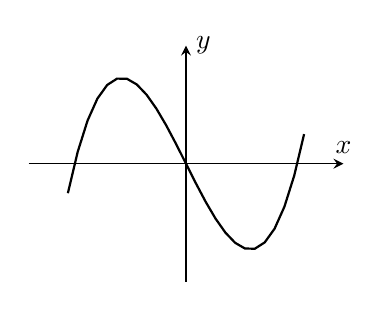
\begin{tikzpicture}[scale=1]
\draw[->,>=stealth,semithick](-2,0)--(2,0)node[above]{$x$};%x軸
\draw[->,>=stealth,semithick](0,-1.5)--(0,1.5)node[right]{$y$};%y軸
\draw[thick,domain=-1.5:1.5] plot(\x,{pow(\x,3)-2*\x});
\end{tikzpicture} 
\end{figure}

実際これは,$X, Y$を実数の集合$\bbR$としたときの関数$f:X \to Y$になっている.
グラフは各$x \in X$に対して唯一の$f(x) \in Y$を割り当てているし,また上の曲線は$\bbR \times \bbR$の部分集合になっていることを確認しよう.

\begin{figure}[h]
\centering
\begin{tikzpicture}[scale=1]
\draw (0,0) ellipse (1 and 1.5);
\node (A) at (0,1.2) {A}; 
\node (B) at (0,0.4) {B}; 
\node (C) at (0,-0.4) {C}; 
\node (D) at (0,-1.2) {D}; 

\draw (-3,0) ellipse (1 and 1.5);
\node (1) at (-3,1) {清}; 
\node (2) at (-3,0) {金}; 
\node (3) at (-3,-1) {銀}; 

\draw[->] (A) -- (1);
\draw[->] (A) -- (3);
\draw[->] (B) -- (2);
\draw[->] (B) -- (3);
\draw[->] (C) -- (1);
% 単射の図

\draw (3,0) ellipse (1 and 1.5);
\node (J) at (3,1) {JP}; 
\node (U) at (3,0) {US}; 
\node (F) at (3,-1) {FR}; 

\draw[->] (A) -- (U);
\draw[->] (B) -- (J);
\draw[->] (C) -- (F);
\draw[->] (D) -- (U);
\end{tikzpicture} 
\caption{関係と関数:左側は1節の表で示した「〜は…に行ったことがある」という二項関係,右側は上表の「〜は…国で生まれた」という関数を図示している.関数においては,ドメインの全ての要素A, B, C, Dに対して,行き先が一つだけ定まっている.}
\end{figure}



\begin{example}[意味論]
関数は哲学でも非常に頻繁に登場する.
ここでは1章の事例2.1で少し見た,言語の意味論をより洗練させてみよう.
一般に\emph{意味論}(semantics)とは,言葉,特に述語論理の言語にその意味を割り当てる作業を指す.
これは,述語論理を構成する項や述語から,その外延(指示対象)の集合$X$への関数を構築することでなされる.
いま,述語論理の個体定項の集合を$C$,一項述語の集合を$P_1$,二項述語の集合を$P_2$・・・と表すことにしよう.
すると求める対応は
\begin{itemize}
 \item 個体定項に対して$X$の要素を対応させる関数 \ \ $f^C: C \to X$
 \item 一項述語に対して$X$の部分集合を対応させる関数 \ \ $f^P_{[1]}: P_1 \to \mcalP(X)$
 \item 二項述語に対して$X$上の関係を対応させる関数 \ \ $f^P_{[2]}: P_2 \to \mcalP(X \times X)$
\end{itemize}
等々の関数によって与えられる.
例えば,個体定項として\{Alice, Bob, Chris, 清水寺, 金閣寺, 銀閣寺\} を持つ言語を考えよう.このときこの意味を与える関数は
\begin{itemize}
 \item これらの定項それぞれには人物や寺社を割り当て
 \item 「〜は人である」という一項述語には,アリス,ボブ,クリスからなる集合を割り当て,
 \item 「〜は...に行ったことがある」という二項述語に対しては1節で定めた関係$R$を割り当てる.
\end{itemize}
このように,言語の意味論を与えるとは,言葉の集合に対してその指示対象の集合(およびその部分集合や関係)を割り当てる関数を構築することである.
\end{example}

\begin{example}[状態]
$3 \times 3$のまるばつゲームを考えよう.
それぞれのマスには,空白(blank),◯,×のどれかが入る.
よって一つの状態(state)には,$3 \times 3$のボード上の一つの関数 $f:\{1, 2, 3\} \times \{1, 2, 3\} \to \{ \text{b, ◯, ×}\}$が対応する.

入力と出力の組み合わせによって,関数は様々な状態を表すことができる.
例えば視覚像は,二次元平面からの色関数$r, g, b:\bbR \times \bbR \to \bbR^+$の組み合わせとして考えられる.
この場合,一つの関数組$(r,g,b)$が,「一枚」の視覚像に対応する(もちろんその圧倒的大多数は何の意味も見いだせないノイズ・砂嵐である).
また3次元空間内の各場所に位置エネルギーを割り当てる関数は,物理学において重力ポテンシャルと呼ばれる.これはいわば各タイムスライスにおける世界における重力の「状態」を表している.
\end{example}


\begin{example}[四次元主義]
\emph{4次元主義}によれば,個物とは4次元時空間内の塊である.
例えばナポレオンは,$t_0=$1769年8月15日から$t_1=$1821年5月5日までの間地球のある部分(主にフランス近辺)を占めた塊(これを時空間ワーム space-time worm と呼ぶ)である.
これを関数によってモデル化してみよう.
時間$T$から3次元空間(簡単のためユークリッド空間$\mathbb{R}^3$とする)の部分集合への関数$I:T \to \mcalP(\mathbb{R}^3)$を考える.
4次元主義において,個体とはこうした関数だと考えられる.
たとえば個体ナポレオンを表す$I_{Np}$は,$I_{Np}(t_0)=$コルシカ島のどこか一部分,$I_{Np}(t_1)=$セントヘレナ島のどこか一部分,であるような関数であり,$t_0 \leq t \leq t_1$であるような$t$に対し$I_{Np}(t)$はナポレオンの人生のある時点でのタイムスライスである.
(吉井達也氏の提案)
\end{example}

\begin{exercise}
上述の4次元主義における個体関数について
 \begin{enumerate}
  \item $t < t_0, t_1 < t$であるような$t$について,関数$I$はどう定義すればよいだろうか.
  \item $T$から$\mcalP(\mathbb{R}^3)$へのどのような関数も個体を定義するといえるだろうか.そうでないとしたら,どんな問題があるだろうか.
 \end{enumerate}
\end{exercise}


\begin{develop}
ただ2つの元からなる集合$\mathbf{2} := \{0, 1\}$を考える.
$X$を任意の集合とし,関数$f:X \to \mathbf{2}$を考えると,この関数$f$は各元$x \in X$に対し0か1を割り当てることによって,$X$の部分集合$A \subset X$と同一視できる.
なぜなら,$f(x)=1$ならこの部分集合に入れ,$f(x)=0$なら入れない,というように,$f$は$A$の選択基準を与えるからだ.
こうした$f$は特性関数(characteristic function)と呼ばれ,$X$からの特性関数全体の集合を$\mathbf{2}^X$と書く,つまり
\[
 \mathbf{2}^X := \{ f|f:X \to \mathbf{2}\}.
\]
一般に,$X$からの特性関数を一つ決めると$X$の部分集合が一つ定まり,逆もまたしかり.
よって,$\mathbf{2}^X$と$\mcalP(X)$は同一視できる.
\end{develop}




\section{写像の合成}
2つの関数$f:X \to Y, g:Y \to Z$の値域と定義域が一致している場合,この2つを連結して関数$g \circ f:X \to Z$をつくることができる.この関数を$f$と$g$の\emph{合成写像}(composition)とよぶ.
具体的に合成写像$g \circ f$は,$x \in X$に対して$g(f(x)) \in Z$を対応させる.
つまり$f$で写した元をさらに$g$で写す.
$f$の後に$g$を適用するのに,$g \circ f$と書くのは一見逆な気がするが,この記法は$g(f(x))$という書き方に合わせてある.

写像の合成は\emph{結合的}(associative)であり,任意の写像$f:W \to X, g:X \to Y, h:Y \to Z$があったとき,$(h \circ g) \circ f = h \circ (g \circ f)$が成り立つ.
つまり$h$と$g$を先に合成したものと$f$を合成しても,$g$と$f$を合成したものに$h$を合成しても,同じ$W$から$Z$への写像ができる.


\begin{figure}[h]
\centering
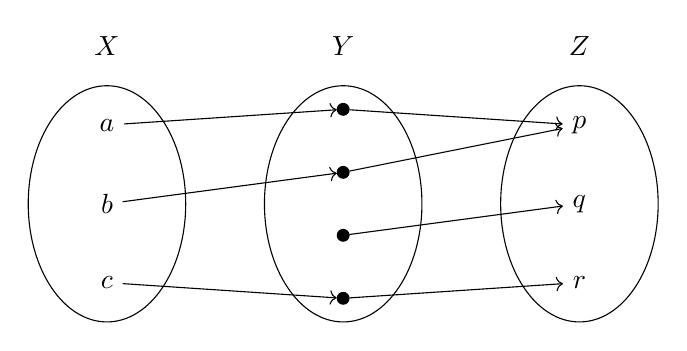
\begin{tikzpicture}
\draw (-3,0) ellipse (1 and 1.5);
\node at (-3,2) {$X$}; 
\node (1) at (-3,1) {$a$}; 
\node (2) at (-3,0) {$b$}; 
\node (3) at (-3,-1) {$c$}; 

\draw (0,0) ellipse (1 and 1.5);
\node at (0,2) {$Y$}; 
\node[draw, circle, fill=black, inner sep=1.5pt] (4) at (0,1.2) {}; 
\node[draw, circle, fill=black, inner sep=1.5pt] (5) at (0,0.4) {}; 
\node[draw, circle, fill=black, inner sep=1.5pt] (6) at (0,-0.4) {}; 
\node[draw, circle, fill=black, inner sep=1.5pt] (7) at (0,-1.2) {}; 

\draw (3,0) ellipse (1 and 1.5);
\node at (3,2) {$Z$}; 
\node (8) at (3,1) {$p$};
\node (9) at (3,0) {$q$};
\node (10) at (3,-1) {$r$};

\draw[->] (1) -- (4);
\draw[->] (2) -- (5);
\draw[->] (3) -- (7);
\draw[->] (4) -- (8);
\draw[->] (5) -- (8);
\draw[->] (6) -- (9);
\draw[->] (7) -- (10);
\end{tikzpicture} 
\caption{関数$f:X \to Y, g:Y \to Z$の合成.$g \circ f$は,$g \circ f (a) = g \circ f (b) =p, g \circ f (c) = r$となるような$X$から$Z$への関数を定めている.}
\end{figure}


\begin{exercise}
上で見た関数$y = f(x) = x^3 -2x$は$\bbR$からそれ自身への関数であり,よって合成$f \circ f$を考えることができる.$f \circ f$を$X$の関数として具体的に書き下せ.
\end{exercise}



\section{像と逆像}

関数$f:X \to Y$は$X$の元を$Y$の元に「飛ばす」が,これを$X$の複数の元に対して行えば,同時に$X$の部分集合に対して$Y$の部分集合を対応させることになる.
関数$f$が$A \subset X$を$Y$に飛ばした先の$Y$の部分集合を,$f$による$A$の\emph{像}(image)とよび,以下のように書く
\[
 f(A) = \{f(x)|x \in A\} 
\]
これは$f(x)$からなる集合なので$Y$の部分集合である.よって$f:X \to Y$は,同時に$f:\mcalP(X) \to \mcalP(Y)$,つまり$X$の部分集合から$Y$の部分集合への関数も自然に伴うことになる.

その逆に,$f$によって$Y$のある部分集合$B \subset Y$に飛ばされる$X$の部分を,$f$による$B$の\emph{逆像}(invarse image)とよび,以下のように書く
\[
 f^{-1}(B) = \{x|f(x) \in B\} 
\]
これは$f(x)$が$B$に入るような$x$の集まりだから,$X$の部分集合である点に注意.
このように,任意の$Y$の部分集合$B$に対して,その逆像$f^{-1}(B)$を考えることができる.
こうした対応づけを$f^{-1}$と書くと,これは$f$とは逆に,$Y$の部分集合から$X$の部分集合への関数$f^{-1}:\mcalP(Y) \to \mcalP(X)$になっている.

この関数への入力として,ある特定の$Y$の要素$y \in Y$(正確にはその一点集合$\{y\}$)を取れば,その逆像は$y$に飛ばされる$X$の値の集合$f^{-1}(y) := \{ x \in X | f(x) = y\}$となる.
そのような$x$は複数あるかもしれない,つまり$f(x) = f(x') = y$となる複数の異なる$x \neq x'$が存在しうるので,これはあくまで$X$の部分集合であることに注意.
例えば上の出生地表では,「$f(x)=\text{アメリカ}$」となる人はAliceとDaveの二人がいるし,$y=x^3-2x$の場合$x=0, \pm \sqrt{2}$のとき$f(x)=0$となる.
よって一般に$f^{-1}$は$Y \to X$への関数には\emph{ならない}(あくまで$\mcalP(X)$への関数である)ことに注意.

\begin{figure}[h]
\centering
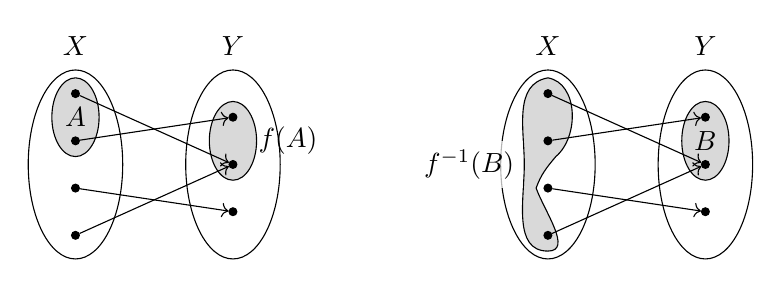
\begin{tikzpicture}[
    dot/.style={draw, circle, fill=black, inner sep=1pt} % 全てのノードに適用されるスタイル
    ]
\begin{scope}
\draw (0,0) ellipse (0.6 and 1.2);
\node at (0,1.5) {$X$}; 
\draw (0,0.6) ellipse (0.3 and .5) [fill=gray!30];
\node at (0,.6) {$A$}; 
\node[dot] (1) at (0,.9) {}; 
\node[dot] (2) at (0,.3) {}; 
\node[dot] (3) at (0,-.3) {}; 
\node[dot] (4) at (0,-.9) {}; 

\draw (2,0) ellipse (0.6 and 1.2);
\node at (2,1.5) {$Y$}; 
\draw (2,0.3) ellipse (0.3 and .5) [fill=gray!30];
\node at (2.7,0.3) {$f(A)$}; 
\node[dot] (a) at (2,.6) {}; 
\node[dot] (b) at (2,0) {}; 
\node[dot] (c) at (2,-.6) {};  
\draw[->] (1) -- (b);
\draw[->] (2) -- (a);
\draw[->] (3) -- (c);
\draw[->] (4) -- (b);
\end{scope} 
\begin{scope}[xshift=6cm]
\draw (0,0) ellipse (0.6 and 1.2);
\node at (0,1.5) {$X$}; 
\draw (0,1.1) to[out=190,in=90] (-.3,0) to[out=270,in=180] (0,-1.1) to[out=0,in=290] (-.15,-.3) to[out=70,in=230] (.1,.1) to[out=40,in=350] (0,1.1) [fill=gray!30];
\node[fill=white, fill opacity=0.7, text opacity=1] at (-1,0) {$f^{-1}(B)$}; 
\node[dot] (1) at (0,.9) {}; 
\node[dot] (2) at (0,.3) {}; 
\node[dot] (3) at (0,-.3) {}; 
\node[dot] (4) at (0,-.9) {}; 

\draw (2,0) ellipse (0.6 and 1.2);
\node at (2,1.5) {$Y$}; 
\draw (2,0.3) ellipse (0.3 and .5) [fill=gray!30];
\node at (2,0.3) {$B$}; 
\node[dot] (a) at (2,.6) {}; 
\node[dot] (b) at (2,0) {}; 
\node[dot] (c) at (2,-.6) {};  
\draw[->] (1) -- (b);
\draw[->] (2) -- (a);
\draw[->] (3) -- (c);
\draw[->] (4) -- (b);
\end{scope}
\end{tikzpicture}
\caption{関数$f:X \to Y$の像(左)と逆像(右).これらが冪集合の間の関数$f:\mcalP(X) \to \mcalP(Y), f^{-1}:\mcalP(Y) \to \mcalP(X)$を与えることを様々な$A \subset X, B \subset Y$で試して確認せよ.} %
\end{figure}


\begin{exercise}
 上の出生地表で,各国の逆像を求めよ.
\end{exercise}

\begin{exercise}
関数の逆像は同値類を与える.
つまり関数$f:X \to Y$が与えらたとき,その逆像の集合
\[
 \{f^{-1}(y) | y \in Y\}
\]
は$X$を分割する.
この分割において同値類をなす関係はどんなものだろう.つまり$a \in X$としたとき,
\[
 [a] = \{x \in X |\dots \}
\]
の「$\dots$」に入るのはどのような条件だろうか.
またこの関係が反射的・対称的・推移的であることを確認せよ.
\end{exercise}


\begin{exercise}
関数$f:X \to Y$としたとき,単元集合$\{x\}$の像$f(\{x\})$はなんだろうか.
\end{exercise}



\begin{exercise}
 任意の関数$f:X \to Y$に対して,$\{x'\} \subset f^{-1}(f(\{x'\}))$であることを示せ.
(ヒント:集合$f^{-1}(f(\{x'\}))$は,逆像の定義より$\{ x | f(x) \in f(\{x'\}) \}$である.これは$x'$を含むか?)
\end{exercise}


\begin{example}
 事例3.2において,世界メイトが同値類をなすことを確認した.
 任意の個物$x \in X$に対して,それが住む世界$w \in W$を返す関数$f:X \to W$を考えると,$x$の世界メイトは$[x] = f^{-1}(f(\{x\}))$として表される.
 これと事例3.2での世界メイト同値類の解釈とを比較せよ.
\end{example}


\begin{example}
\label{eg:essence}
$X$を個物の集合,$E$を\emph{本質}(essense)の集合とすれば,関数$e:X \to E$は各個物にその本質を対応させる.
これが個物の分類を与えることを確認せよ.
この関数の像の逆像$e^{-1} (e(x))$は何を意味するだろうか.
%逆に,個物を分類することは,本質を想定することと同じだろうか.
\end{example}


\section{全射と単射}
\ref{sec:relation_kinds}節では,反射性や対称性など,色々な関係のあり方を見た.
同様に,関数にも制約を加えることで種類を考えることができる.
これらの種別は大変重要なので,最初はこんがらがるかもしれないがぜひ頭に叩き込んでおいてほしい.

関数$f:X \to Y$が\emph{全射}(surjection)であるとは,$Y$のすべての元が対応する$X$を持つということ,より正確に言えば$f(X)=Y$となることである.
つまり$X$を関数で飛ばすことで$Y$の全域をカバーすることができる.ここから全射は「上からの」(onto)写像ともいわれる.

関数$f:X \to Y$が\emph{単射}(injection)であるとは,異なる$X$の元は必ず異なる$Y$の元に飛ばされる,つまり$x \neq x'$なら$f(x) \neq f(x')$が成り立つということである.
あるいは単射とはその逆像$f^{-1}(y)$が常に単元集合になる関数,といってもよい.
重複を防ぐためには当然,$Y$の元の個数は$X$の元の個数より多くなければならない.
ここから単射は「中への」(into)写像ともいわれる.

全射かつ単射であるような関数は,\emph{全単射}(bijection)といわれる.
全単射$f:X \to Y$があるとき,$X$の元と$Y$の元は一対一に対応する.
よって全単射のことを\emph{1対1写像}(one-to-one mapping)ともいう.

\begin{figure}[h]
\centering
\begin{minipage}{0.32\textwidth}
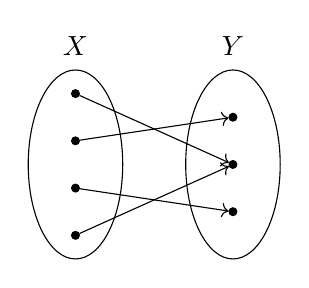
\begin{tikzpicture}[
    dot/.style={draw, circle, fill=black, inner sep=1pt} % 全てのノードに適用されるスタイル
    ]
\draw (0,0) ellipse (0.6 and 1.2);
\node at (0,1.5) {$X$}; 
\node[dot] (1) at (0,.9) {}; 
\node[dot] (2) at (0,.3) {}; 
\node[dot] (3) at (0,-.3) {}; 
\node[dot] (4) at (0,-.9) {}; 

\draw (2,0) ellipse (0.6 and 1.2);
\node at (2,1.5) {$Y$}; 
\node[dot] (a) at (2,.6) {}; 
\node[dot] (b) at (2,0) {}; 
\node[dot] (c) at (2,-.6) {};  
\draw[->] (1) -- (b);
\draw[->] (2) -- (a);
\draw[->] (3) -- (c);
\draw[->] (4) -- (b);
\end{tikzpicture} 
\end{minipage}
\begin{minipage}{0.32\textwidth}
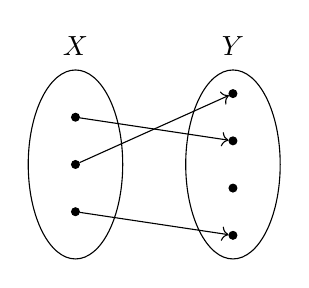
\begin{tikzpicture}[
    dot/.style={draw, circle, fill=black, inner sep=1pt} % 全てのノードに適用されるスタイル
    ]
\draw (0,0) ellipse (0.6 and 1.2);
\node at (0,1.5) {$X$}; 
\node[dot] (1) at (0,.6) {}; 
\node[dot] (2) at (0,0) {}; 
\node[dot] (3) at (0,-.6) {}; 

\draw (2,0) ellipse (0.6 and 1.2);
\node at (2,1.5) {$Y$}; 
\node[dot] (a) at (2,.9) {}; 
\node[dot] (b) at (2,.3) {}; 
\node[dot] (c) at (2,-.3) {};  
\node[dot] (d) at (2,-.9) {};  
\draw[->] (1) -- (b);
\draw[->] (2) -- (a);
\draw[->] (3) -- (d);
\end{tikzpicture}
\end{minipage}
\begin{minipage}{0.32\textwidth}
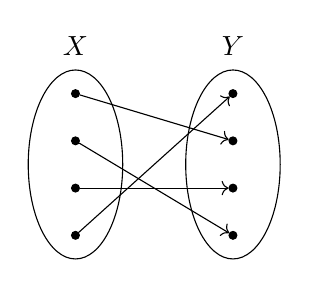
\begin{tikzpicture}[
    dot/.style={draw, circle, fill=black, inner sep=1pt} % 全てのノードに適用されるスタイル
    ]
\draw (0,0) ellipse (0.6 and 1.2);
\node at (0,1.5) {$X$}; 
\node[dot] (1) at (0,.9) {}; 
\node[dot] (2) at (0,.3) {}; 
\node[dot] (3) at (0,-.3) {}; 
\node[dot] (4) at (0,-.9) {}; 

\draw (2,0) ellipse (0.6 and 1.2);
\node at (2,1.5) {$Y$}; 
\node[dot] (a) at (2,.9) {}; 
\node[dot] (b) at (2,.3) {}; 
\node[dot] (c) at (2,-.3) {};  
\node[dot] (d) at (2,-.9) {};  
\draw[->] (1) -- (b);
\draw[->] (2) -- (d);
\draw[->] (3) -- (c);
\draw[->] (4) -- (a);
\end{tikzpicture} 
\end{minipage}
\caption{全射(左),単射(中),全単射(右)関数の例.}
\end{figure}


$f:X \to Y$が全単射であるとき,$Y$のすべての元$y$に対して,$f(x)=y$となるような$x \in X$が必ず一つだけ存在する.
よって$y$をそのような$x$に対応させるような関数を考えることができる.
これを$f$の\emph{逆写像}(inverse map/function)とよび,$f^{-1}$と表す.つまり
\[
 f^{-1}:Y \to X, \hspace{2em} y \mapsto x \text{ such that } f(x)=y
\]
である.
記号は上の節でみた逆像と同じだが,内容は違うので混同しないように.
逆像は冪集合$\mcalP(Y)$から冪集合$\mcalP(X)$への関数で,あらゆる関数について考えることができる.
一方,逆写像は$Y$から$X$への関数で,これは$f$が全単射であるときのみ存在する.
なぜならそのとき,任意の$y \in Y$に対しその逆像$f^{-1}(y)$は$X$の単元集合になり,これを元と同一視することで関数$f^{-1}(y)$の値と考えることができるからだ.

\begin{exercise}
 逆写像を持つためには$f$は単射でなければならないことは上で納得できたと思う.ではなぜそれは全射である必要があるのだろうか.
\end{exercise}

\begin{exercise}
$X/R$を集合$X$上の同値関係$R$による商集合だとすると,任意の$x \in X$にその同値類$[x]$を対応させる関数$f:X \to X/R, x \mapsto [x]$を考えることができる.
この関数は全射だろうか.単射だろうか.また一般にそうでないとしたら,どんなときにそうなるだろうか.
\end{exercise}


% \begin{example}
% % \label{eg:supervenience}
% %  $X$を個物の集合,$Y$と$Z$を性質の集合とし,$f_Y:X \to Y, f_Z:X \to Z$を物にそれぞれの性質を割り当てる関数とする.
% % 例えば$X$を(各時点の)人の集合,$Y, Z$をそれぞれその心的/物理的状態と考えれば,$f_Y$はその人の心的状態を表す.
% % $Y$が$Z$に\emph{付随}(supervene)するとは,$Y$における差異が必ず$Z$における差異を含意すること,つまり任意の$x, x' \in X$について$f_Y(x) \neq f_Y(x')$なら$f_Z(x) \neq f_Z(x')$が成立することである.
% % この付随性を,$Y$と$Z$の間の関数として表すことができるだろうか.
% % またこの関数はどのような性質を持つだろうか.
% \end{example}

% \begin{exercise}
%  $\bfV$を性質の集合とし,$V, V' \in \bfV$に対し$V \preceq V'$によって「性質$V$が$V'$にsuperveneする」という二項関係を表すものとする.この二項関係は(1)反射的,(2)対称的,(3)非対称的,(4)反対称的,(5)推移的だろうか,それぞれ考えよ.
% \end{exercise}


\section{無限集合}
集合には色々なものがある.
Jackson 5と五大湖は当然違う集合だ(片方は人,もう片方は湖を元として持つ).
しかし両者もともに5つの元からなる,という点においては同じである.
この数としての同じさは,2つの集合の間の全単射(1対1対応)によって保証される.
つまりJackie $\leftrightarrow$ スペリオル湖,Tito $\leftrightarrow$ ミシガン湖$\dots$というような対応づけを「ニックネーム」だと思えば,5大湖でもってJackson兄弟を代表させることが可能だ(ちょっとダサいけど).
このように2つの集合$X, Y$のあいだに全単射が存在するとき,$X$と$Y$は\emph{同等}であるといい,$X \sim Y$と書く.
全単射の性質より,これは集合の間の同値関係を与える.

\begin{attn}
 2つの集合が同等であるからといって同一であるとは限らない(Jackson 5と五大湖はどう考えても同一ではない).
\end{attn}

集合$X$の「大きさ」を,その\emph{濃度}ないし\emph{基数}(cardinality)といい,$|X|$で表す.
有限集合の場合,濃度とは元の数にほかならない.例えば集合としてのJackson 5の濃度は5である.
これは集合$\{1, 2, 3, 4, 5\}$と同等であるということである.
もったいぶって書けば,有限集合とは,ある自然数$n$を用いて $\{1, 2, \dots, n\}$と表される集合と同等である,つまりその間に全単射が存在するということである(細かいことをいえば,空集合も有限集合に含まれる).

一方,自然数全体$\bbN$や実数全体$\bbR$は無限集合であり,そのような形では書けない.
無限集合には,我々の直観に反するような面白い性質がある.
有限集合の場合,真部分集合の濃度はもとの集合の濃度より当然小さい.
しかし無限集合には,その部分であって,なおかつ同等であるようなものが存在する.
例えば$\bbN$を自然数の集合,$\bbN_E$を偶数の集合とすると,当然$\bbN_E \subsetneq \bbN$である.
しかし$\phi::n \mapsto 2n$を考えると,これは$\bbN, \bbN_E$の間の全単射を与える(確認せよ).
よって$|\bbN| = |\bbN_E|$であり,両者は同等である.
両者は元の一対一対応という意味では同等だが,包含関係においてはそうではない.
これが上で濃度を「大きさ」とカギカッコ付きで述べた理由である.

逆に無限集合を,「それ自身と同等であるような真部分集合を持つ集合」と定義することもできる.

$\bbN$と同等な集合を\emph{可算無限集合}(countably infinite set)という.
上で見たように$\bbN_E$は可算無限であるし,同様に奇数の集合も可算無限である.
また実は,整数の集合$\bbZ$や有理数の集合$\bbQ$も可算無限であり,$\bbN$との間に一対一対応をつけることができる(明らかに$\bbN \subsetneq \bbZ \subsetneq \bbQ$なのにも関わらず!).

では実数の集合$\bbR$もそうかというと,実はこれは可算ではない.
実数と自然数の間には一対一対応がつけられないことは,カントールによる\emph{対角線論法}によって示された.
アイデアは画期的だが,証明自体は難しくないので気になる人は調べてみてほしい.
この結果が意味するのは,自然数も実数も無限にあるのだが,実数のほうがより「大きい」無限である,つまり無限にも種類があるということである.
$\bbR$のように,$\bbN$と同等でない無限集合を,\emph{非可算(無限)集合}(uncountable set)という.
つまり一個一個数え上げれないほどたくさんある,ということだ.

\begin{develop}
 $\bbN$の濃度を$\aleph_0$と書き,「アレフゼロ」と読む($\aleph$はヘブライ文字の最初の字).
一方$\bbR$の濃度は$\aleph_1$と書かれる.
実は$\bbN$の冪集合$2^\bbN$の濃度は実数と同じ$\aleph_1$になることが知られている.
では,$\aleph_0$と$\aleph_1$の中間の濃度,つまり「自然数よりは大きいが実数よりは小さい」集合は存在するだろうか?
このような集合は存在しない,という主張が有名な\emph{連続体仮説}(continuum hypothesis)である.
ちなみにこの仮説は,標準的な集合論のもとでは証明も反証もできない(つまり独立である)ということが知られている.
\end{develop}


\end{document}